% ==========================================================
% Lecture Notes: Oscillation / SHM (with "hand-drawn" TikZ)
% Goal: drawings that look as close as possible to your page.
% Compile with: pdflatex (or lualatex)
% ==========================================================

\documentclass[11pt]{article}

\usepackage{amsmath, amssymb}
\usepackage{physics}
\usepackage{siunitx}
\usepackage{geometry}
\geometry{margin=1in}

\usepackage{tikz}
\usepackage{pgfplots}
\pgfplotsset{compat=1.18}
\usetikzlibrary{
  arrows.meta,
  decorations.pathmorphing,
  decorations.markings,
  calc,
  positioning
}

% ---------------------------
% Hand-drawn / sketchy styles
% ---------------------------
\tikzset{
  sk/.style={
    line width=0.9pt,
    decorate,
    decoration={random steps, segment length=4pt, amplitude=0.75pt}
  },
  skthin/.style={
    line width=0.7pt,
    decorate,
    decoration={random steps, segment length=4pt, amplitude=0.55pt}
  },
  axis/.style={-{Stealth[length=3.0mm]}, line width=0.9pt},
  force/.style={-{Stealth[length=3.0mm]}, line width=0.9pt},
  note/.style={font=\small},
  tinyNote/.style={font=\footnotesize},
}

\title{14. Oscillation (Class Notes)}
\author{}
\date{}

\begin{document}
\maketitle

\vspace{-0.75em}

\section*{Equilibrium}

\begin{itemize}
\item \textbf{Equilibrium:} $\sum \vec F = 0$.
\item This does \emph{not} mean “not moving.” You can have $\sum \vec F = 0$ and still move at constant velocity.
\item \textbf{Stable equilibrium:} if displaced, the system experiences a restoring tendency back toward the equilibrium point.
\end{itemize}

\begin{center}
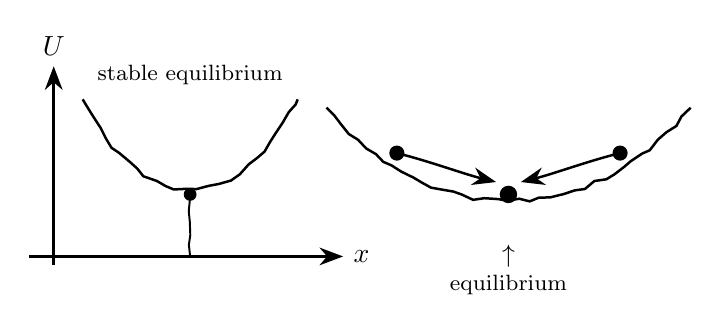
\begin{tikzpicture}[scale=1.05]

% --- Left: potential well U vs x with stable equilibrium ---
\begin{scope}[shift={(0,0)}]
  \draw[axis] (-0.1,-0.1) -- (-0.1,2.3) node[above] {$U$};
  \draw[axis] (-0.4,0.0) -- (3.4,0.0) node[right] {$x$};

  % Well curve (hand-drawn-ish)
  \draw[sk] (0.25,1.9) .. controls (1.0,0.45) and (2.1,0.45) .. (2.85,1.9);

  % equilibrium marker (minimum)
  \fill (1.55,0.75) circle (2.2pt);
  \draw[skthin] (1.55,0.0) -- (1.55,0.75);

  \node[tinyNote] at (1.55,2.2) {stable equilibrium};
\end{scope}

% --- Right: "ball in a bowl" with arrows like your sketch ---
\begin{scope}[shift={(5.4,0.2)}]
  % bowl
  \draw[sk] (-2.2,1.6) .. controls (-1.0,0.1) and (1.0,0.1) .. (2.2,1.6);
  % ball at bottom
  \fill (0,0.55) circle (3pt);

  % side positions + curved arrows (show motion back and forth)
  \fill (-1.35,1.05) circle (2.6pt);
  \fill ( 1.35,1.05) circle (2.6pt);

  % arrows pointing "back toward center"
  \draw[force] (-1.35,1.05) .. controls (-0.95,0.95) and (-0.55,0.80) .. (-0.15,0.70);
  \draw[force] ( 1.35,1.05) .. controls ( 0.95,0.95) and ( 0.55,0.80) .. ( 0.15,0.70);

  \node[note] at (0,-0.2) {$\uparrow$};
  \node[tinyNote] at (0,-0.55) {equilibrium};

\end{scope}
\end{tikzpicture}
\end{center}

\vspace{-0.5em}

\section*{Period, Frequency, and “Cycle”}

\begin{itemize}
\item \textbf{Period} $T$: time for \emph{one full cycle} (seconds).
\item \textbf{Frequency} $f$: number of cycles per second (Hz).
\end{itemize}

\[
f = \frac{1}{T},\qquad T = \frac{1}{f},\qquad 1\ \text{Hz} = 1\,\text{s}^{-1}.
\]

\begin{center}
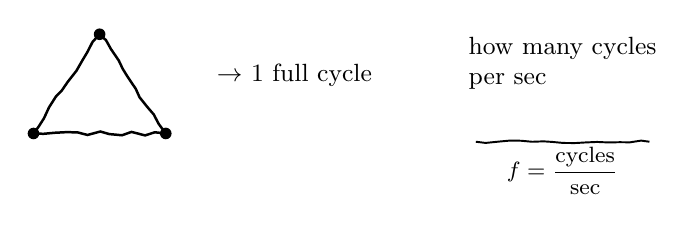
\begin{tikzpicture}[scale=1.05]

% --- little triangle "one full cycle" doodle ---
\begin{scope}[shift={(0,0)}]
  \draw[sk] (0,0) -- (1.6,0) -- (0.8,1.2) -- cycle;
  \fill (0,0) circle (2pt);
  \fill (1.6,0) circle (2pt);
  \fill (0.8,1.2) circle (2pt);
  \node[note, right] at (2.1,0.7) {$\rightarrow$ 1 full cycle};
\end{scope}

% --- right-side: "how many cycles per sec" scribble idea ---
\begin{scope}[shift={(6.4,0.1)}]
  \node[align=left, note] at (0,0.75) {how many cycles\\per sec};
  \draw[skthin] (-1.05,-0.2) -- (1.05,-0.2);
  \node[tinyNote] at (0,-0.55) {$f=\dfrac{\text{cycles}}{\text{sec}}$};
\end{scope}

\end{tikzpicture}
\end{center}

\subsection*{Quick unit check (like your line)}
If you complete $N$ cycles in $1$ second, then
\[
f = \frac{N\ \text{cycles}}{1\ \text{s}}.
\]
If one cycle takes $T$ seconds, then
\[
f = \frac{1\ \text{cycle}}{T\ \text{s}}=\frac{1}{T}\ \text{Hz}.
\]

\subsection*{Radio station meaning}
A radio station at \SI{100}{MHz} means the electromagnetic field oscillates
\[
100\times 10^{6}\ \text{times per second}.
\]

\section*{Many Examples of SHM}

SHM (simple harmonic motion) is the kind of oscillation produced by a \textbf{restoring influence} that is proportional to displacement (for small displacements). The result is sinusoidal motion.

\begin{center}
\begin{tikzpicture}[scale=1.0]

% Axes for the big sine sketch
\draw[axis] (0,-0.3) -- (0,3.1);
\draw[axis] (-0.3,1.4) -- (11.4,1.4);

% Sine-like curve (hand-drawn style)
\draw[sk]
  plot[smooth, samples=150, domain=0:11]
  (\x, {1.4 + 1.25*sin(deg(0.55*\x - 0.7))});

% Mark three points like your circles on the curve
\foreach \x in {2.2,5.5,8.8}{
  \filldraw[white] (\x, {1.4 + 1.25*sin(deg(0.55*\x - 0.7))}) circle (3.2pt);
  \draw[skthin] (\x, {1.4 + 1.25*sin(deg(0.55*\x - 0.7))}) circle (3.2pt);
}

% little arrow at the right end
\draw[force] (10.8, {1.4 + 1.25*sin(deg(0.55*10.8 - 0.7))})
          -- (11.25,{1.4 + 1.25*sin(deg(0.55*11.25 - 0.7))});

\node[note, anchor=west] at (0.2,2.85) {Many examples for SHM};

% Bottom doodles (little "U" arcs under the axis)
\begin{scope}[shift={(0.0,0.0)}]
  \foreach \x in {1.0, 3.2, 5.4, 7.6, 9.8}{
    \draw[sk] (\x,0.55) .. controls (\x+0.55,0.05) and (\x+1.10,0.05) .. (\x+1.65,0.55);
  }
\end{scope}

\end{tikzpicture}
\end{center}

\section*{Why are sine waves and SHM related?}

One clean way to see the connection: \textbf{uniform circular motion projected onto a line gives sinusoidal motion.}
That’s the idea behind your small circle doodles.

\begin{center}
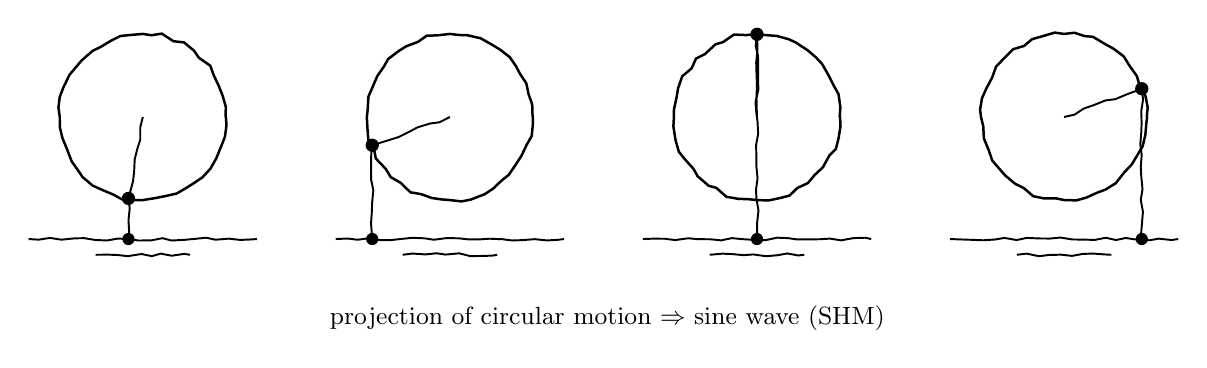
\begin{tikzpicture}[scale=1.0]

% Four snapshots: circle with a point + projection to a line
\foreach \X/\ang in {0/260, 3.9/200, 7.8/90, 11.7/20}{
  \begin{scope}[shift={(\X,0)}]
    % circle
    \draw[sk] (0,0) circle (1.05);

    % baseline (like notebook line)
    \draw[skthin] (-1.45,-1.55) -- (1.45,-1.55);

    % radius to point
    \draw[skthin] (0,0) -- ({1.05*cos(\ang)},{1.05*sin(\ang)});
    \fill ({1.05*cos(\ang)},{1.05*sin(\ang)}) circle (2.4pt);

    % projection down to line
    \draw[skthin] ({1.05*cos(\ang)},{1.05*sin(\ang)}) -- ({1.05*cos(\ang)},-1.55);
    \fill ({1.05*cos(\ang)},-1.55) circle (2.2pt);

    % small slanted "ground" mark under each (matches your vibe)
    \draw[skthin] (-0.6,-1.75) -- (0.6,-1.75);
  \end{scope}
}

\node[note] at (5.9,-2.55) {projection of circular motion $\Rightarrow$ sine wave (SHM)};

\end{tikzpicture}
\end{center}

\section*{Summary (matches your page)}
\begin{itemize}
\item Equilibrium: $\sum \vec F=0$ (can still be moving).
\item Stable equilibrium gives a restoring tendency $\Rightarrow$ oscillation.
\item Period $T$ = seconds per cycle; frequency $f$ = cycles per second; $f=1/T$.
\item Many physical systems (near stable equilibrium) approximate SHM $\Rightarrow$ sinusoidal motion.
\item A geometric reason for sine: projection of uniform circular motion.
\end{itemize}

\end{document}
